%============================================================================%
%
%	DOCUMENT DEFINITION
%
%============================================================================%

\input{glyphtounicode}
\pdfgentounicode=1

%we use article class because we want to fully customize the page and don't use a cv template
\documentclass[10pt,A4]{article}	


%----------------------------------------------------------------------------------------
%	ENCODING
%----------------------------------------------------------------------------------------

% we use utf8 since we want to build from any machine
\usepackage[utf8]{inputenc}		

%----------------------------------------------------------------------------------------
%	LOGIC
%----------------------------------------------------------------------------------------

% provides \isempty test
\usepackage{xstring, xifthen}

%----------------------------------------------------------------------------------------
%	FONT BASICS
%----------------------------------------------------------------------------------------

% some tex-live fonts - choose your own

%\usepackage[defaultsans]{droidsans}
%\usepackage[default]{comfortaa}
%\usepackage{cmbright}
\usepackage[default]{raleway}
%\usepackage{fetamont}
%\usepackage[default]{gillius}
%\usepackage[light,math]{iwona}
%\usepackage[thin]{roboto} 

% set font default
\renewcommand*\familydefault{\sfdefault} 	
\usepackage[T1]{fontenc}

% more font size definitions
\usepackage{moresize}

%----------------------------------------------------------------------------------------
%	FONT AWESOME ICONS
%---------------------------------------------------------------------------------------- 

% include the fontawesome icon set
\usepackage{fontawesome}

% use to vertically center content
% credits to: http://tex.stackexchange.com/questions/7219/how-to-vertically-center-two-images-next-to-each-other
\newcommand{\vcenteredinclude}[1]{\begingroup
\setbox0=\hbox{\includegraphics{#1}}%
\parbox{\wd0}{\box0}\endgroup}

% use to vertically center content
% credits to: http://tex.stackexchange.com/questions/7219/how-to-vertically-center-two-images-next-to-each-other
\newcommand*{\vcenteredhbox}[1]{\begingroup
\setbox0=\hbox{#1}\parbox{\wd0}{\box0}\endgroup}

% icon shortcut
\newcommand{\icon}[3] { 							
	\makebox(#2, #2){\textcolor{maincol}{\csname fa#1\endcsname}}
}	

% icon with text shortcut
\newcommand{\icontext}[4]{ 						
	\vcenteredhbox{\icon{#1}{#2}{#3}}  \hspace{2pt}  \parbox{0.9\mpwidth}{\textcolor{#4}{#3}}
}

% icon with website url
\newcommand{\iconhref}[5]{ 						
    \vcenteredhbox{\icon{#1}{#2}{#5}}  \hspace{2pt} \href{#4}{\textcolor{#5}{#3}}
}

% icon with email link
\newcommand{\iconemail}[5]{ 						
    \vcenteredhbox{\icon{#1}{#2}{#5}}  \hspace{2pt} \href{mailto:#4}{\textcolor{#5}{#3}}
}

\newcommand{\iconegithub}[5]{                         
    \vcenteredhbox{\icon{#1}{#2}{#5}}  \hspace{2pt} \href{#4}{\textcolor{#5}{#3}}
}


%----------------------------------------------------------------------------------------
%	PAGE LAYOUT  DEFINITIONS
%----------------------------------------------------------------------------------------

% page outer frames (debug-only)
% \usepackage{showframe}		

% we use paracol to display breakable two columns
\usepackage{paracol}

% define page styles using geometry
\usepackage[a4paper]{geometry}

% remove all possible margins
\geometry{top=1cm, bottom=1cm, left=1cm, right=1cm}

\usepackage{fancyhdr}
\pagestyle{empty}

% space between header and content
% \setlength{\headheight}{0pt}

% indentation is zero
\setlength{\parindent}{0mm}

%----------------------------------------------------------------------------------------
%	TABLE /ARRAY DEFINITIONS
%---------------------------------------------------------------------------------------- 

% extended aligning of tabular cells
\usepackage{array}

% custom column right-align with fixed width
% use like p{size} but via x{size}
\newcolumntype{x}[1]{%
>{\raggedleft\hspace{0pt}}p{#1}}%


%----------------------------------------------------------------------------------------
%	GRAPHICS DEFINITIONS
%---------------------------------------------------------------------------------------- 

%for header image
\usepackage{graphicx}

% use this for floating figures
% \usepackage{wrapfig}
% \usepackage{float}
% \floatstyle{boxed} 
% \restylefloat{figure}

%for drawing graphics		
\usepackage{tikz}				
\usetikzlibrary{shapes, backgrounds,mindmap, trees}

%----------------------------------------------------------------------------------------
%	Color DEFINITIONS
%---------------------------------------------------------------------------------------- 
\usepackage{transparent}
\usepackage{color}

% primary color
\definecolor{maincol}{RGB}{ 0, 36, 88 }

% accent color, secondary
% \definecolor{accentcol}{RGB}{ 250, 150, 10 }

% dark color
\definecolor{darkcol}{RGB}{ 70, 70, 70 }

% light color
\definecolor{lightcol}{RGB}{220,220,220}


% Package for links, must be the last package used
\usepackage[hidelinks]{hyperref}

% returns minipage width minus two times \fboxsep
% to keep padding included in width calculations
% can also be used for other boxes / environments
\newcommand{\mpwidth}{\linewidth-\fboxsep-\fboxsep}
	


%============================================================================%
%
%	CV COMMANDS
%
%============================================================================%

%----------------------------------------------------------------------------------------
%	 CV LIST
%----------------------------------------------------------------------------------------

% renders a standard latex list but abstracts away the environment definition (begin/end)
\newcommand{\cvlist}[1]{
    \begin{itemize}
        \setlength{\itemsep}{2pt}   % Reduces space between items
        \setlength{\parskip}{0pt}   % Reduces space between paragraphs within items
        #1
    \end{itemize}
}

\usepackage{enumitem} % Add this line to your preamble if not already included

\newcommand{\sidebarcvlist}[1]{
    \begin{itemize}[left=0pt, labelindent=0pt, labelsep=5pt, listparindent=\parindent]
        #1
    \end{itemize}
}

%----------------------------------------------------------------------------------------
%	 CV TEXT
%----------------------------------------------------------------------------------------

% base class to wrap any text based stuff here. Renders like a paragraph.
% Allows complex commands to be passed, too.
% param 1: *any
\newcommand{\cvtext}[1] {
	\begin{tabular*}{1\mpwidth}{p{0.98\mpwidth}}
		\parbox{1\mpwidth}{#1}
	\end{tabular*}
}

%----------------------------------------------------------------------------------------
%	CV SECTION
%----------------------------------------------------------------------------------------

% Renders a a CV section headline with a nice underline in main color.
% param 1: section title
\newcommand{\cvsection}[1] {
	\vspace{4pt}
	\cvtext{
		\textbf{\Large{\textcolor{darkcol}{#1}}}\\[-4pt]
		\textcolor{maincol}{ \rule{0.1\textwidth}{2pt} } \\
	}
}

%----------------------------------------------------------------------------------------
%	META SKILL
%----------------------------------------------------------------------------------------

% Renders a progress-bar to indicate a certain skill in percent.
% param 1: name of the skill / tech / etc.
% param 2: level (for example in years)
% param 3: percent, values range from 0 to 1
\newcommand{\cvskill}[3] {
	\begin{tabular*}{1\mpwidth}{p{0.72\mpwidth}  r}
 		\raggedright\textcolor{black}{\textbf{#1}} & \textcolor{maincol}{#2}\\
	\end{tabular*}%
	
	\hspace{4pt}
	\begin{tikzpicture}[scale=1,rounded corners=2pt,very thin]
		\fill [lightcol] (0,0) rectangle (1\mpwidth, 0.1);
		\fill [maincol] (0,0) rectangle (#3\mpwidth, 0.1);
  	\end{tikzpicture}%
}

\newcommand{\cvskillcompact}[3] {
	\begin{tabular*}{1\mpwidth}{p{0.72\mpwidth}  r}
 		\raggedright\textcolor{black}{\textbf{#1}} & \textcolor{maincol}{#2}\\
	\end{tabular*}%
	
	\hspace{4pt}
	\begin{tikzpicture}[scale=1,rounded corners=2pt,very thin]
		\fill [lightcol] (0,0) rectangle (1\mpwidth, 0.1);
		\fill [maincol] (0,0) rectangle (#3\mpwidth, 0.1);
  	\end{tikzpicture}%
}

%----------------------------------------------------------------------------------------
%	 CV EVENT
%----------------------------------------------------------------------------------------

% Renders a table and a paragraph (cvtext) wrapped in a parbox (to ensure minimum content
% is glued together when a pagebreak appears).
% Additional Information can be passed in text or list form (or other environments).
% the work you did
% param 1: time-frame i.e. Sep 14 - Jan 15 etc.
% param 2:	 event name (job position etc.)
% param 3: Customer, Employer, Industry
% param 4: Short description
% param 5: work done (optional)
% param 6: technologies include (optional)
% param 7: achievements (optional)
\newcommand{\cvevent}[7] {
	
	% we wrap this part in a parbox, so title and description are not separated on a pagebreak
	% if you need more control on page breaks, remove the parbox
    % \parbox{\mpwidth}{
    %     \begin{tabular*}{1\mpwidth}{@{} p{\dimexpr0.59\mpwidth-\tabcolsep} r @{}}
    %         \textcolor{black}{\textbf{#2}} & \colorbox{maincol}{\makebox[0.42\mpwidth]{\textcolor{white}{#1}}} \\
    %         \textcolor{maincol}{\textbf{#3}} & \\
    %     \end{tabular*}\\[8pt]

    %     \ifthenelse{\isempty{#4}}{}{
    %         \cvtext{#4}
    %     }
    % }
    \parbox{\mpwidth}{
      \begin{tabular*}{1\mpwidth}{p{0.59\mpwidth}  r}
          \textcolor{black}{\large{\textbf{#2}}} & \colorbox{white}{\makebox[0.52\mpwidth]{\textcolor{black}{#1}}} \\
          \textcolor{maincol}{\textbf{#3}} & \\
      \end{tabular*}\\[0pt]
    
      \ifthenelse{\isempty{#4}}{}{
          \cvtext{#4}
      }
    }    
	% \parbox{\mpwidth}{
    %   \begin{tabular*}{1\mpwidth}{p{0.59\mpwidth}  r}
    %       \textcolor{black}{\textbf{#2}} & \colorbox{white}{\makebox[0.42\mpwidth]{\textcolor{black}{#1}}} \\
    %       \textcolor{maincol}{\textbf{#3}} & \\
    %   \end{tabular*}\\[8pt]
    
    %   \ifthenelse{\isempty{#4}}{}{
    %       \cvtext{#4}
    %   }
    % } 

	\ifthenelse{\isempty{#5}}{}{
		\vspace{0pt}
		{#5}
	}

	\ifthenelse{\isempty{#6}}{}{
		\vspace{0pt}
		\cvtext{\textbf{Technologies:}}
		{#6}
	}

	\ifthenelse{\isempty{#7}}{}{
		\vspace{4pt}
		\cvtext{\textbf{Achievements:}}
		{#7}
	}
	\vspace{12pt}
}

%----------------------------------------------------------------------------------------
%	 CV META EVENT
%----------------------------------------------------------------------------------------

% Renders a CV event on the sidebar
% param 1: title
% param 2: subtitle (optional)
% param 3: customer, employer, etc,. (optional)
% param 4: info text (optional)
\newcommand{\cvmetaevent}[4] {


	\ifthenelse{\isempty{#2}}{}{
	\textcolor{darkcol} {\cvtext{\textbf{#2}} }
	}

	\ifthenelse{\isempty{#3}}{}{
		\cvtext{{ \textcolor{darkcol} {#3} }}\\
	}

	\cvtext{#4}\\[14pt]
}

%---------------------------------------------------------------------------------------
%	QR CODE
%----------------------------------------------------------------------------------------

% Renders a qrcode image (centered, relative to the parentwidth)
% param 1: percent width, from 0 to 1
\newcommand{\cvqrcode}[1] {
	\begin{center}
		
\includegraphics[width={#1}\mpwidth]{qrcode}
	\end{center}
}


%============================================================================%

%%
%
%	DOCUMENT CONTENT
%
%
%
%============================================================================%
\begin{document}
\columnratio{0.3}
\setlength{\columnsep}{2.2em
}\setlength{\columnseprule}{3pt}
\colseprulecolor{lightcol}
\begin{paracol}{2}
\begin{leftcolumn}
%---------------------------------------------------------------------------------------
%	META IMAGE + info
%----------------------------------------------------------------------------------------
%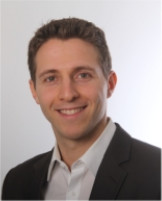
\includegraphics[width=\linewidth]{untitled.jpg}	%trimming relative to image size



\vfill\null
\cvsection{Contact}
	
\icontext{MapMarker}{12}{Sweden/world}{black}\\[6pt]
\icontext{MobilePhone}{12}{+33 6 75 10 87 20}{black}\\[6pt]
\iconemail{Envelope}{12}{ha.lagrange9000@gmail.com}{ha.lagrange9000@gmail.com}{black}\\[6pt]
\iconegithub{Github}{12}{github.com/Dedalum}{https://github.com/Dedalum}{black}\\


%---------------------------------------------------------------------------------------
%	META SKILLS
%----------------------------------------------------------------------------------------
\cvsection{Skills}

\makebox[0pt][l]{%
% \hspace*{-5pt}
\begin{tabular*}{1\linewidth}{p{0.18\linewidth} >{\raggedright\arraybackslash}p{0.75\linewidth}}
	\textcolor{black}{\LARGE{+++}} & \textcolor{black}{Python, SQL, git }\\[5pt]
	\textcolor{black}{\LARGE{++}} & \textcolor{black}{Golang, Ansible, InfluxDB/Grafana, ELK stack, Bash/UNIX}\\[5pt]
	\textcolor{black}{\LARGE{+}} & \textcolor{black}{Tailwind, Nuxt/Vue, Jenkins, AWS/GCP, K8s}\\[5pt]
	\textcolor{black}{\textbf{Other}} & \textcolor{black}{Agile methods, cross-team communication, customer support, marketing basics, web 3 practitioner}\\[5pt]  
\end{tabular*}%
}

\cvsection{Languages}

\begin{tabular*}{1\linewidth}{p{0.33\linewidth} >{\raggedright\arraybackslash}p{0.67\linewidth}}
	\textcolor{black}{\textbf{Fluent}} & \textcolor{black}{English, French}\\[5pt]  
	\textcolor{black}{\textbf{Basics}} & \textcolor{black}{German, Swedish, Spanish}\\[5pt]
\end{tabular*}%


%---------------------------------------------------------------------------------------
%	EDUCATION
%----------------------------------------------------------------------------------------
\cvsection{Education}

\cvmetaevent
{}
{Master, IT \& CS}
{Université de Technologie de Troyes - Troyes, France}
{Networking and telecommunication, specializing in cryptography and infosec}

\cvmetaevent
{}
{Exchange}
{University of Waterloo\\Waterloo, Canada, Fall 2014}
{Faculty of mathematics, computer science program: computer \& information security, CS, graph theory}

% -------
% Extra
% -------

\cvsection{Interests}
{\sidebarcvlist{
    \item Web 3 supporter, Fintech \& AI applications
    \item Business \& marketing \& startups
    \item Literature, beer brewing,\\adrenalin
}}

%---------------------------------------------------------------------------------------
%	CERTIFICATION
%----------------------------------------------------------------------------------------
% \newpage
% \cvsection{CERTIFICATIONS}

% \cvmetaevent
% {LPIC 1 - Linux administrator}
% {}
% {}
% {Certificate issued by the Linux Professional Institute to prove abilities in Linux administration}


\end{leftcolumn}
\begin{rightcolumn}
%---------------------------------------------------------------------------------------
%	TITLE  HEADER
%----------------------------------------------------------------------------------------
\fcolorbox{white}{white}{\begin{minipage}[c][1cm][c]{1\mpwidth}
	\begin {center}
		\textbf{ \Large{ \textcolor{black}{ Hugues Lagrange } }  | \large{ \textcolor{black} {Developer} } }
	\end {center}
\end{minipage}} \\[1pt]
\vspace{-6pt}

%---------------------------------------------------------------------------------------
%	PROFILE
%----------------------------------------------------------------------------------------
\cvtext{Flexible and adaptive tech person looking for challenges, exciting products and good team spirit, with specific experience in Python and Golang in the web3 \& fintech industries. Devops and automation mindset, problem solver, open-minded. Into product development and marketing.
}\\[8pt]

%---------------------------------------------------------------------------------------
%	WORK EXPERIENCE
%----------------------------------------------------------------------------------------
\cvsection{Professional experience}
\cvevent
	{March 24 - Sept 24, 7 mo}
	{Senior developer (XP x2)}
	{Tada - Remote/Dubai, UAE}
	{Ta-da is a web 3 startup building a micro-tasking platform in the process of being fully decentralized. Tokenomics include the TADA token distributed on MVX,
    used through the application for user rewards, customers purchasing micro-tasks and other gamification aspects.}
    {\cvlist{
        \item Backend lead developer, cross-team planning with the designer, frontend and sales teams
        \item Challenges: dealing with a big legacy code-base in a rapidly evolving environment, high availability requirements on the API \& DB, organisational issues
        \item \textbf{Technologies:} Python FastAPI (REST), AWS Lambdas, AWS Aurora RDS \& MySQL, Redis, Gitlab CI, Grafana metrics (MySQL, MongoDB)
    }}
    {}
    {}

\cvevent
    {Nov 23 - Feb 24}
    {Side project: language webapp}
    {\href{https://maitre-hanguk.com}{Maître Hanguk}}
    {FastAPI, Nuxt 3/Vue 3, Tailwind, Postgres, Ansible, Stripe, Traefik, Web marketing \& SEO}
    {}
    {}
    {}
\cvevent
    {Feb 23 - May 23, 4 mo}
    {Software \& product development}
    {PDF Toolkit API - Remote, France}
    {Built a SaaS company providing an API to generate various types of PDF documents including receipts and reports in a team of 2. \\[4pt]
    Techs/skills: FastAPI, Vue 3, Tailwind, Postgres, Ansible, Traefik, Web marketing \& SEO}
    {}
    {}
    {}

\cvevent
	{Apr 20 - Jul 23, 3 yr 4 mo}
	{Python developer}
	{Linxo - Remote/France}
	{Linxo is a French fintech startup aggregating banking data for individuals and offering services of accounting and business finance for businesses.}
    {\cvlist{
        \item Cross-team design and implementation of features and business logic for banking and financial data gathering, GDPR environment
        \item Regular meetings with French banks for issues solving and feature developments, level 3 customer support
        \item \textbf{Technologies:} Python, PostgreSQL, Java/Go, Jenkins, ELK stack, Grafana metrics (Postgres, Influxdb), Bash
    }}
    {}
    {}

% \vfill\null
\cvevent
	{May 17 - Aug 18, 1 yr 4 mo}
    {Software developer - Golang \& Python}
    {Snuk - Berlin, Germany}
    {Early-stage startup building an IoT infrastructure platform for smart buildings.}
    {\cvlist{
        \item Design of distributed systems, implementation and installation of on-premise IoT infrastructures and cloud architectures
        \item Direct product development with the customers and remote \& on-site support with the factories management and workers
        \item \textbf{Technologies:} Golang \& Python, Bash, Postgres, MongoDB, GCP, Docker, Ansible, TIGK stack, IoT (BLE, MQTT, Raspberry Pi)
    }}
    {}
    {}

% \vfill\null
% \cvevent
%     {Mar 16 - Sep 16, 6 mo}
%     {IT security/admin intern}
%     {Freespee AB - Uppsala, Sweden}
%     {}
%     % {Freespee is a real time conversation cloud for marketers. AWS, ELK stack \& Redis, Ansible, OpenVPN server, Linux, Bash \& Python scripting.}
%     % I worked as an intern in the engineering team, in Uppsala, Sweden, performing system administration tasks with a focus on information security. Along my different projects were}
%     % {\cvlist{
%     %     \item Deploying an ELK stack for central log management with a Redis buffer in an AWS VPC (25 VMs)
%     %     \item Preparing an office firewall based on Debian (iptables scripts, Suricata IDS, OpenVPN bridge, VLANs, DHCP and local DNS)
%     %     \item Installing an OpenVPN server for a secure remote access to the AWS VPC
%     %     \item Research and setup of a ”chatops” solution using Slack and Errbot, Jenkins, Ansible and Docker 
%     % }}
% 	{}
%     {}
% 	{}

% % \vfill\null
% \cvevent
%     {Feb 15 - Jul 15, 6 mo}
%     {\{System administrator, PHP developer - Jymeo, France}}
%     % {Jymeo - Nantes, France}
%     {}
%     % {JYMEO is an internet/marketing start-up. OVH cloud, ELK stack, Ansible, OpenVPN server, Linux, Bash \& Python scripting.}
%     {}
%      % We followed the Scrum method. I deployed and worked on the ELK suite for analyzing server logs, deployed OpenVPN servers and backup scripts, firewalls (iptables, fail2ban, NAXSI), secured Wordpress websites.}
%     % {\cvlist{
%     %     \item Setting up new servers (Virtual machines running Debian 8, with providers OVH/RunAbove) with web-servers (Nginx, Apache)
%     %     \item Level 3 support
%     % }}
%     {}
%     {}
%     {}

% hotfixes to create fake-space to ensure the whole height is used
% \mbox{}
% \vfill
% \mbox{}
% \vfill
% \mbox{}
% \vfill
% \mbox{}
\end{rightcolumn}
\end{paracol}
\end{document}

